\section{Det tekniske bindeleddet: «AquaFeed Manifold»}
\label{sec:innovasjonen}

En melketankbil er konstruert for rørtransport mellom gård og meieri, ikke for manuell utlevering til allmennheten. For å transformere en melkebil til et operativt distribusjonspunkt på under fem minutter, har gruppen utviklet det mekaniske bindeleddet \textbf{«AquaFeed Manifold»} (figur~\ref{fig:tapperigg}). Dette utgjør prosjektets sentrale mekaniske innovasjon.

\begin{figure}[htbp]
    \centering
    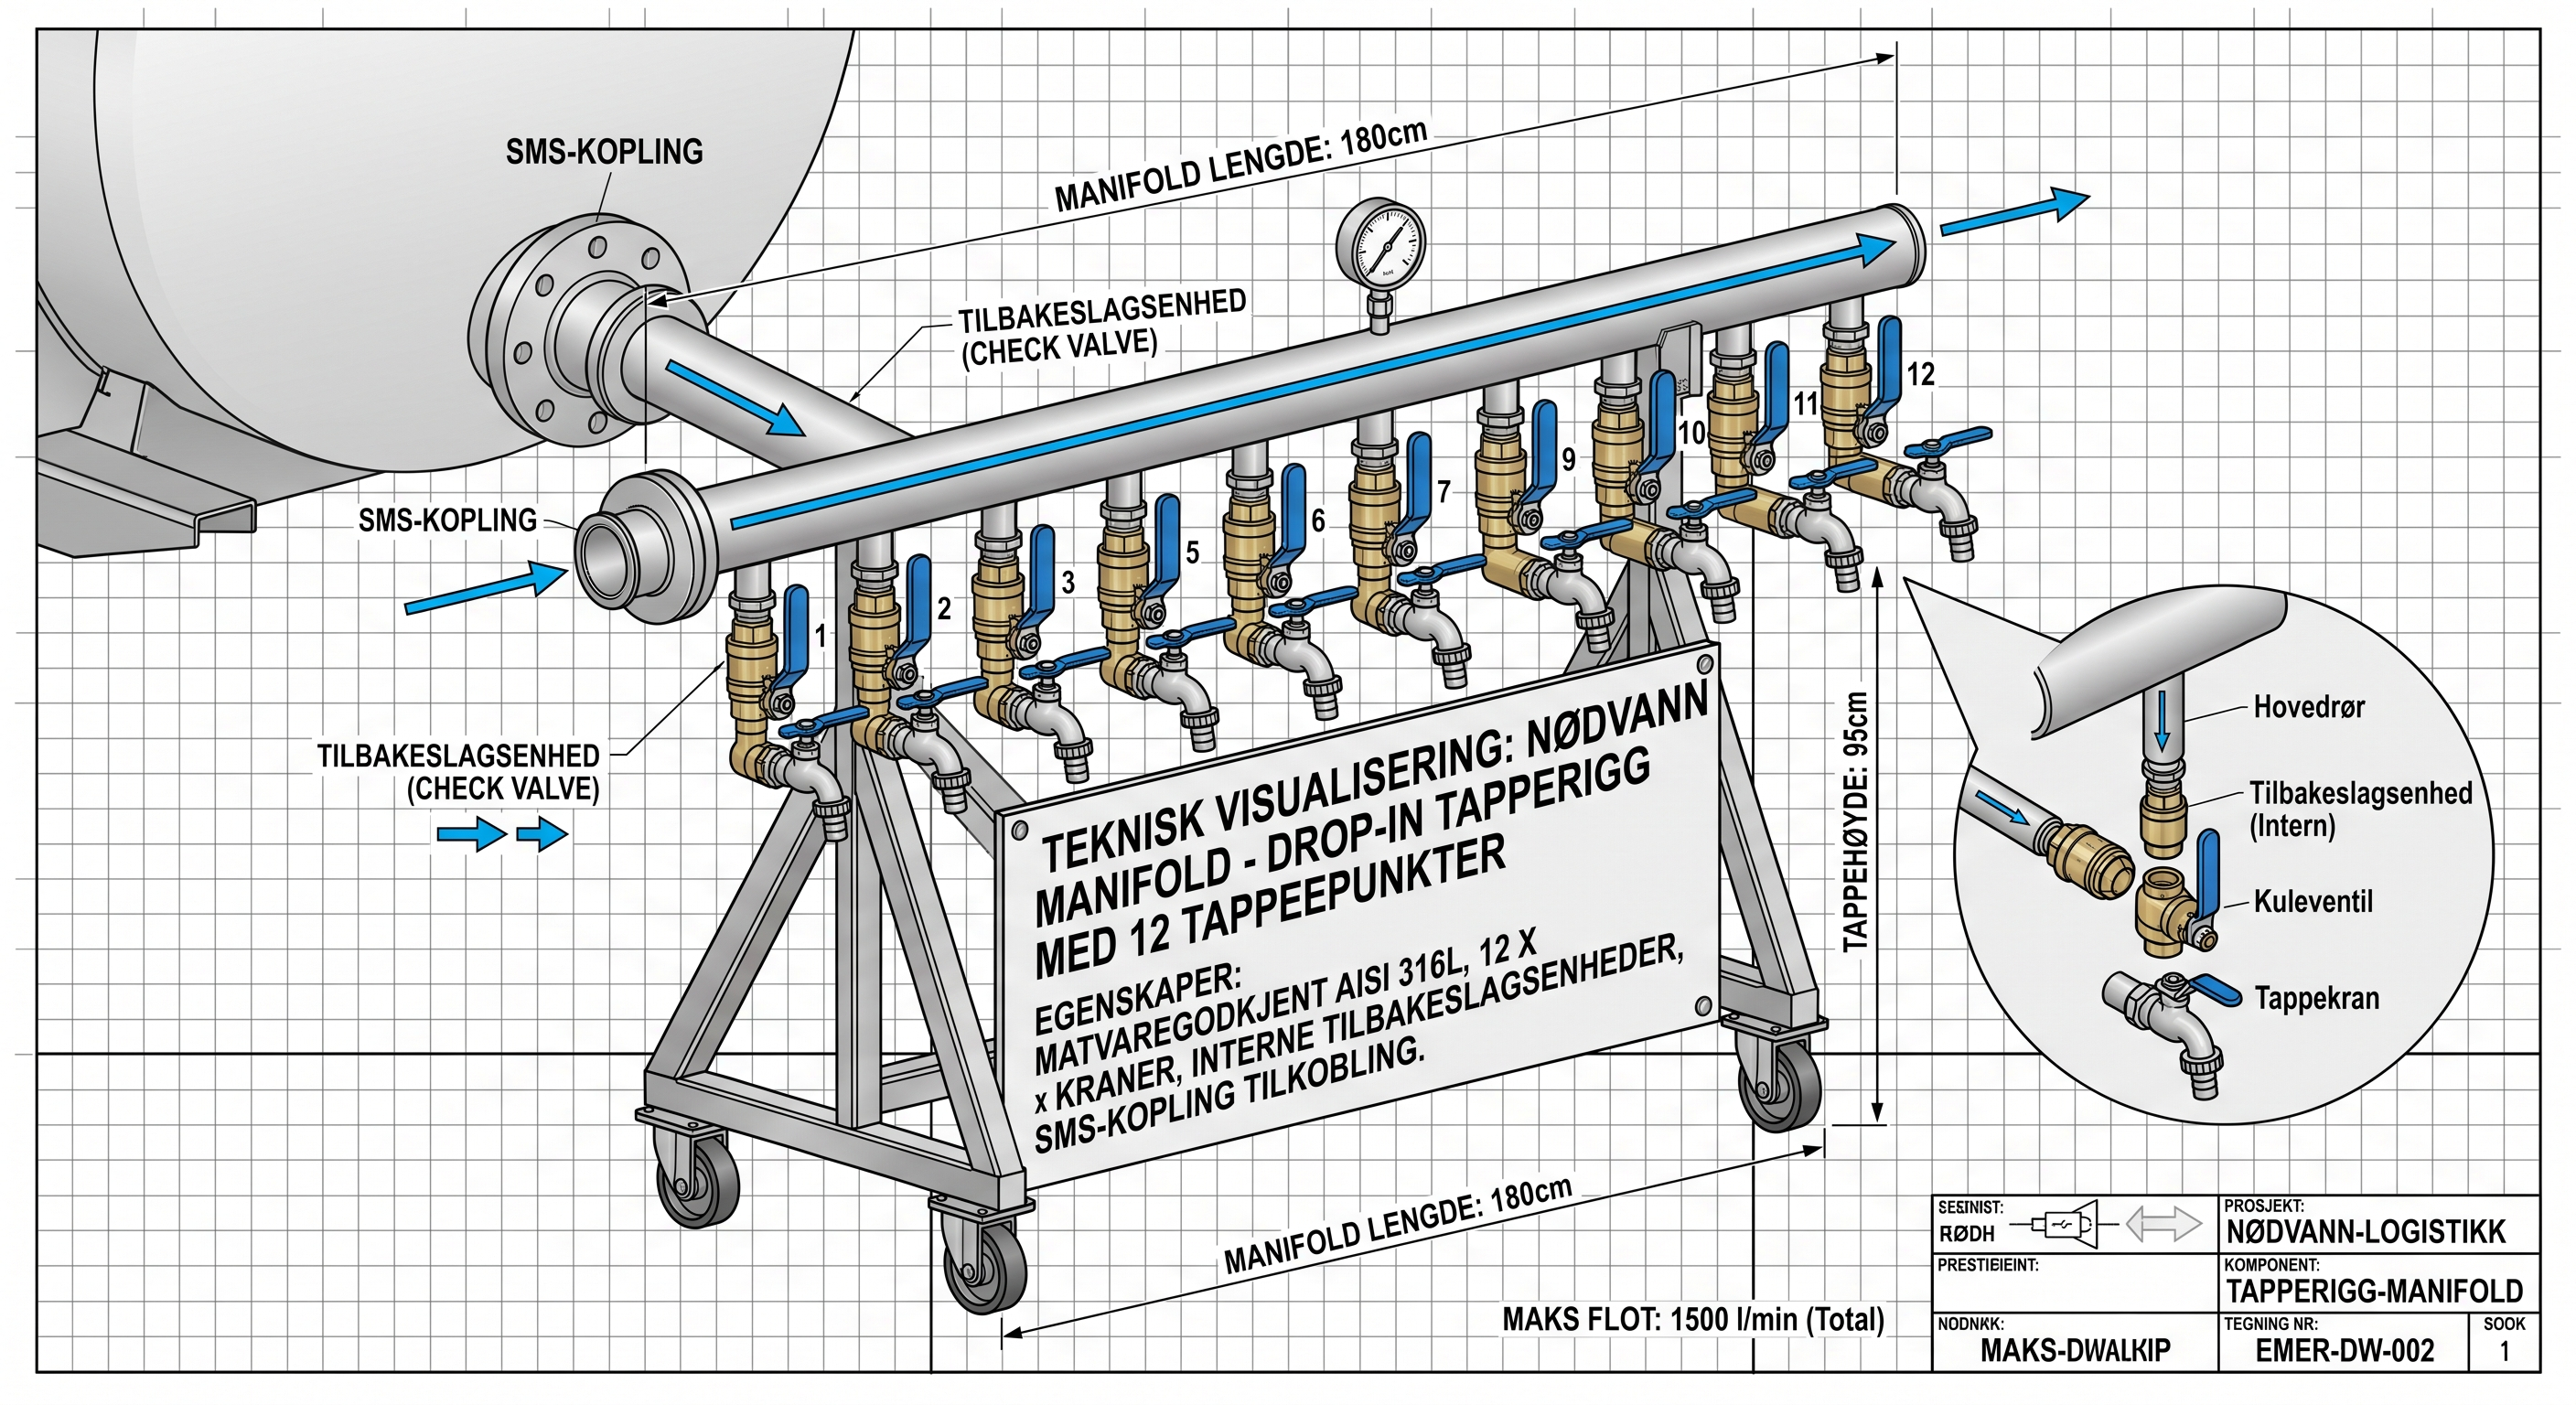
\includegraphics[width=0.92\textwidth]{Figures/Tapperigg.jpg}
    \caption{Den egenutviklede «AquaFeed Manifold»-tapperiggen montert på melkebilens bakre utløp. Modulær oppbygging med 10 parallelle tappepunkter, tilbakeslagsventiler, integrert trykkreduksjon og sammenleggbar støtteramme.}
    \label{fig:tapperigg}
\end{figure}

\subsection{Mekanisk konstruksjon og grensesnitt}
Norske melkebiler benytter sanitære koblinger iht. \textsc{sms} 1145 eller \textsc{din} 11851. Riggen fabrikkeres i elektropolert syrefast stål (\textsc{aisi} 316L):
\begin{itemize}[leftmargin=1.5em, itemsep=0.2em]
    \item \textbf{Verktøyløs hurtigkobling:} Riggen festes direkte til bilens \textsc{dn}65/\textsc{dn}76 bunnutløp via en standard \textsc{sms}-mutter med \textsc{epdm}-pakning. Montasjen utføres av sjåføren på under to minutter.
    \item \textbf{Ergonomisk støtteramme:} En integrert, sammenleggbar ramme i rørstål felles ut ved ankomst, avlaster utløpsventilen og plasserer kranene i arbeidshøyde (\SI{90}{\centi\meter}). Under transport lagres den i bilens sideskap.
\end{itemize}

\subsection{Beskyttelse mot krysskontaminering og tilbakesug}
For å eliminere smittefare fra befolkningens kanner har manifolden tre fysiske barrierer:
\begin{enumerate}[leftmargin=1.5em, itemsep=0.15em]
    \item \textbf{Fjærbelastede tilbakeslagsventiler:} Hver av de 10 tappekranene har en tilbakeslagsventil (\textit{non-return}) som stenger momentant ved trykkfall, slik at tilbakesug inn i tanken er fysisk umulig.
    \item \textbf{Berøringsfri geometri:} Tappedysene er skråstilt \ang{45} nedover med fri høyde over dryppristen, hvilket forhindrer kontakt med medbrakte kanner.
    \item \textbf{Flow- og trykkontroll:} En integrert membranventil regulerer trykket til et laminært arbeidstrykk på \num{1.5}--\SI{2.0}{\bar}. En 10-liters beholder fylles på 15--20 sekunder uten sprut.
\end{enumerate}

\subsection{Vinterdrift og universelt adaptersett}
For å sikre drift ved minusgrader er manifolden utstyrt med en integrert \SI{24}{\volt} selvbegrensende varmekabel (\SI{150}{\watt}) koblet til bilens strømuttak, samt hurtigtømmende bunnkraner for sekundrask drenering.

For oppkobling mot eksterne vannkilder medfølger et adaptersett i syrefast stål:
\begin{itemize}[leftmargin=1.5em, itemsep=0.2em]
    \item Overganger fra \textsc{sms}/\textsc{din} til brannvesenets Nor-lås type 1/2 og Storz B/C.
    \item Integrert \SI{100}{\micro\meter} partikkelfilter som fanger opp rust og sedimenter før tanken fylles.
\end{itemize}

\subsection{«Den siste meteren»: Sivil forurensningsbarriere}
Sterilt tankvann forringes dersom befolkningen tapper på urene bøtter. «Den siste meteren» sikres gjennom to tiltak:
\begin{itemize}[leftmargin=1.5em, itemsep=0.2em]
    \item \textbf{Sterile foldekanistere:} Sivilforsvaret og Røde Kors deler ut forhåndslagret, sammenleggbare 10-liters næringsmiddelgodkjente foldekanistere (\textsc{bpa}-frie).
    \item \textbf{Desinfeksjonssluse:} Innbyggere passerer en sluse med håndsprit og overflatedesinfeksjon for kanner før tapping.
\end{itemize}

\subsection{Kostnadskalkyle og nasjonal beredskapsreserve}
Riggen krever ingen elektronisk styring og kan serieproduseres rimelig:
\begin{itemize}[leftmargin=1.5em, itemsep=0.2em]
    \item \textbf{Enhetskostnad:} Fabrikasjon i syrefast stål (\textsc{aisi} 316L) inkludert ventiler, adaptersett og varmekabel er kalkulert til \num{15000}--\SI{25000}{NOK} per enhet.
    \item \textbf{Nasjonal reserve:} En reserve på 50 rigger koster ca. \SI{1.0}{MNOK}. Ved å forhåndslagre rigger ved landets 15 største meierier sikres nasjonal dekning med responstid under to timer.
\end{itemize}
